%Phone 
%open chapters on any page, final removes formatting marks
%avoid conflicts with hyperref by loading before documentclass
\RequirePackage{setspace}

\documentclass[11.75pt,openany,final]{memoir}
\makepagenote
\title{The Discoverer's Digest}
%place graphics package first to avoid conflicts (weird page sizes)
\usepackage{graphicx}
\usepackage{wrapfig}

% package to remove 'Figure x.x' with the \caption*{foo} option
\usepackage[labelformat=empty]{caption}

%\usepackage[paperwidth=70.9mm, paperheight=143.6mm, hmargin={1cm, 1cm},vmargin={1.2cm, 1.25cm}]{geometry}
% New setup
% setstocksize{height}{width}
\setstocksize{216mm}{137mm}
\settrimmedsize{216mm}{137mm}{*}
\settypeblocksize{216mm}{137mm}{*}
\setlrmarginsandblock{24.0mm}{24.0mm}{*}
\setulmarginsandblock{27mm}{27mm}{*}
%\marginparmargin{2mm}
% memoir: finalize the page changes
\checkandfixthelayout

\usepackage{microtype}

% \usepackage{marginnote}
%\usepackage{wrapfig}
%\setbeforesecskip{2mm}
% \setaftersecskip{2mm}
%\setSindent{0pt}

% TYPEFACE PROPERTIES
%--------------------
% fontspec system for typeface definitions
\usepackage{fontspec,xunicode,polyglossia}

%NOTE: good discussion of fonts: https://tex.stackexchange.com/questions/352804/setmainfont-vs-fontspec
%letter spacing

%fontspec font selection
\setmainfont{LinuxLibertineG}[
BoldFont = LinuxLibertineGB,
ItalicFont = LinuxLibertineGI,
BoldItalicFont = LinuxLibertineGZI,
SlantedFont = LinLibertineSlantedZ,
BoldSlantedFont = LinLibertineSlantedZ,
SmallCapsFont = LinLibertineCapitals
]
\setmonofont{LinLibertine_M}
\setsansfont{LiberationSans}


\makeatletter
%\g@addto@macro\chapnamefont{\sffamily} 
%\g@addto@macro\chapnumfont{\sffamily}  
%\g@addto@macro\chaptitlefont{\sffamily}
%\makeatother

% PAGE PROPERTIES
%----------------
%% common ligatures
%TODO: add more ligatures
\usepackage{newunicodechar}
\newunicodechar{ff}{ff}
\newunicodechar{fi}{fi}
\newunicodechar{fl}{fl}
\newunicodechar{ffi}{ffi}
\newunicodechar{ffl}{ffl}
%% end of common ligatures

% multiple columns (bullet lists, etc.)
\usepackage{multicol}

% set the leading
%better as it leaves margin note spacing alone
\setstretch{1.20}

%flexible margin notes
\usepackage{marginnote}
\renewcommand*{\marginfont}{\color{gray!80!black}\tiny\itshape\setstretch{0.9}}
% End notes
%\usepackage{enotez}
%\setenotez{
%  list-name=Credits
  % split=chapter,
  % split-heading={\chaptermark{#1}}
%}

% CHAPTER PROPERTIES
%-------------------

%chapter page style
\makechapterstyle{plroman}{
\renewcommand\printchaptername{}
\renewcommand\printchapternum{\color{red!70!black}\centering\MakeUppercase{\fontsize{.75in}{1in}\selectfont\romannumeral\thechapter}\color{Black}}
\renewcommand\afterchaptertitle{\vskip0.25\midchapskip\vskip\midchapskip\hrule\vskip0.15\midchapskip\vskip\midchapskip}
}

% Use this chapter style
\chapterstyle{plroman}

% Drop first letter of each chapter
\usepackage{lettrine}

% more text sizes (ssize & HUGE)
\usepackage[10pt]{moresize}

% Precise colors
\usepackage[dvipsnames,svgnames,table]{xcolor}

%story splash images
\usepackage[pages=some,placement=top]{background}

% PDF has priority over PNG (for size reasons) when declaring an extensionless
% \includegraphics
\DeclareGraphicsExtensions{.jpg,.pdf,.png}
%bar
% PAGE HEADER PROPERTIES
% -----------------------
\nouppercaseheads
\makepagestyle{mystyle}
% \makeevenhead{mystyle}{\itshape\thetitle}{}{\scshape\MakeLowercase\rightmark}
% \makeoddhead{mystyle}{}{}{\scshape\MakeLowercase\leftmark}
% page numbers to the inside for easier electronic page number navigation (don't
% need to move eyes back-and-forth)
\makeevenfoot{mystyle}{}{}{\thepage}{}
\makeoddfoot{mystyle}{\thepage}{}{}{}
\makepsmarks{mystyle}{%
  \createmark{chapter}{left}{nonumber}{}{}}

\pagestyle{mystyle}

\usepackage[absolute]{textpos}

% get rid of section period in page header
% \def\sectionmark#1{\markboth{#1}{}}
\def\sectionmark#1{\markboth{#1}{#1}}

% SECTION/SUBSECTION STYLE
% --------------------------
\setsecheadstyle{\color{red!70!black}\Large\scshape\raggedright}
\setsubsecheadstyle{\color{red!70!black}\large\scshape\raggedright}
\setsubsubsecheadstyle{\color{red!70!black}\normalsize\scshape\raggedright}
\setbeforesecskip{-1.5ex plus -.5ex minus -.2ex}
\setaftersecskip{1.3ex plus .2ex}
\setbeforesubsecskip{-1.25ex plus -.5ex minus -.2ex}
\setaftersubsecskip{1ex plus .2ex}

%only use chapters in TOC
\settocdepth{chapter}
\renewcommand{\thesection}{}
\renewcommand{\thesubsection}{}

% USE TIKZ FOR DOT CONVERSION
%(not using this as I converted dot SVG's to PDF)
%\usepackage{tikz}
%\usetikzlibrary{snakes,arrows,shapes}
%\usepackage{amsmath}
\usepackage{lscape}

% BETTER REFERENCES
% `on the next page,' etc.
\usepackage{varioref}

% include full-page PDF's
\usepackage{pdfpages}

% source code listing
\usepackage{listings}
\lstset{
  basicstyle=\ssmall\ttfamily,
  columns=fullflexible,
  frame=single,
  breaklines=true,
  postbreak=\mbox{\textcolor{red}{$\hookrightarrow$}\space}
}
\usepackage{parskip}
\setlength{\parindent}{8pt}

% LINK PROPERTIES
%-----------------
\usepackage[pdfversion=1.7,
    pdfauthor={D. Cooper Stevenson},
    pdftitle={The Discoverer's Digest},
    pdfsubject={Interactive Fiction},
    pdfkeywords={Interactive Fiction, Parser, TADS3, Inform, Interactivity},
    pdfproducer={Latex with hyperref},
    pdfcreator={XeLatex}]{hyperref} % Improves typography
\hypersetup{
    colorlinks=true, %Color links instead of ugly boxes
    linkcolor={red!50!black}, %Color of internal links
    citecolor={gray!70!black}, %Color of citations
    urlcolor={red!50!black}, %Color for external hyperlinks
    % urlcolor={BrickRed},
    linktoc=all,
    pdfcenterwindow=true,
  }
\usepackage{attachfile2}
\renewcommand\thefootnote{\textcolor{red!70!black}{\arabic{footnote}}}

\begin{document}
% COVER
%------
%clear the page
\aliaspagestyle{chapter}{empty}

% create a `fake' chapter for title page
\chapter*{}

%define a 'textblock' for the cover image & place image inside cover
\begin{textblock*}{70.9mm}(0mm,0mm)
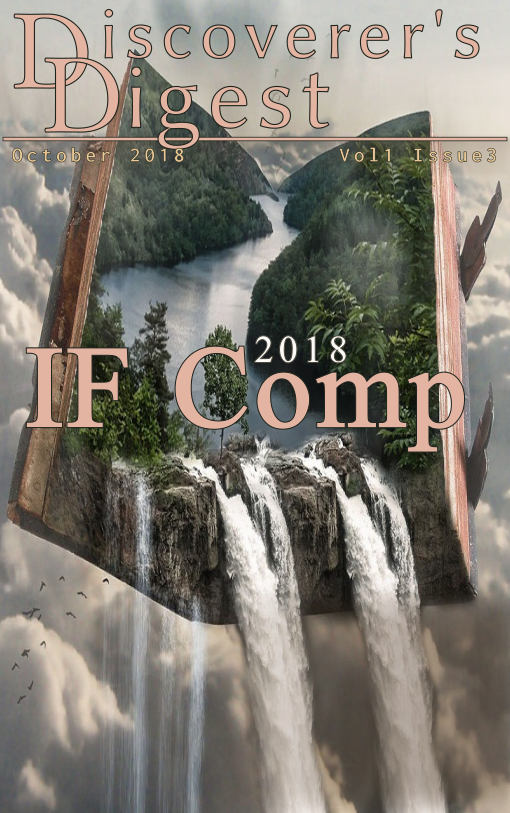
\includegraphics[width=\paperwidth]{./media/images/cover}
\end{textblock*}
\thispagestyle{empty}\clearpage %clear header
  %background image for TOC
  \backgroundsetup{
    scale=1,
    color=black,
    opacity=0.35,
    angle=0,
    contents={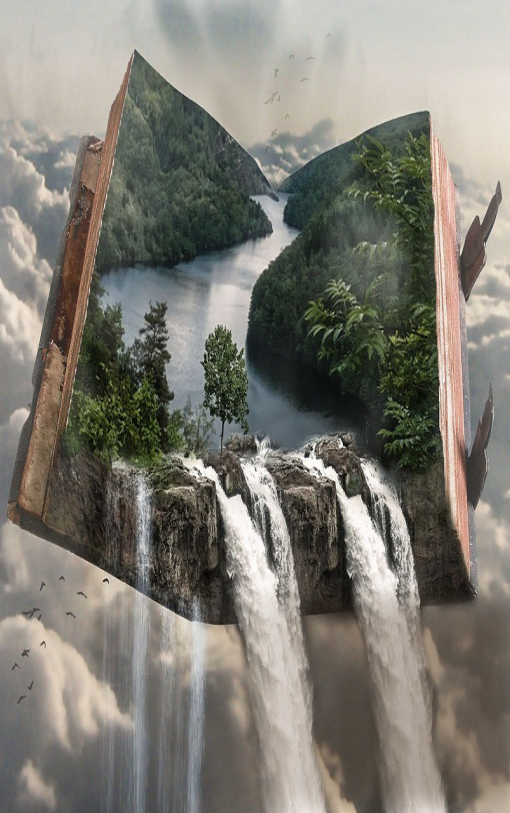
\includegraphics[width=1.01\paperwidth, height=1.01\paperheight,keepaspectratio]{./media/images/cover_splash}}
  }
  \BgThispage
  \tableofcontents*
  \noindent\LARGE{\textbf{Credits}}\medbreak
  \hrule
%  \noindent\rule{9cm}{0.4pt}%watch
  \smallskip
  \noindent\large{\color{red!50!black}{\textbf{Creator\,/\,Graphics\,/\,Author: D. Cooper
        Stevenson}}}\\
  \noindent\small{Cooper Stevenson dedicates himself to enabling fulfilling
    human experiences through the aesthetic use of technology. He lives with his
    wife, \emph{Deanna} and his two cats, \emph{Tiberius} and \emph{Augustus}.}\\ \\
  \noindent\large{\color{red!50!black}{\textbf{Editor: Peter M.J. Gross}}}\\
  \noindent \small{Peter is an editor and online content
  specialist who has been entertained by interactive fiction since "\emph{Nord and
  Bert Couldn't Make Head or Tail of It}." He had to resort to a walkthrough in
  order to complete \emph{Trinity}, and he could never figure out \emph{A Mind Forever
    Voyaging}.}

\thispagestyle{empty} %clear header
\newpage
% First Article
\chapter*{}
\begin{textblock*}{70.9mm}(0mm,0mm)
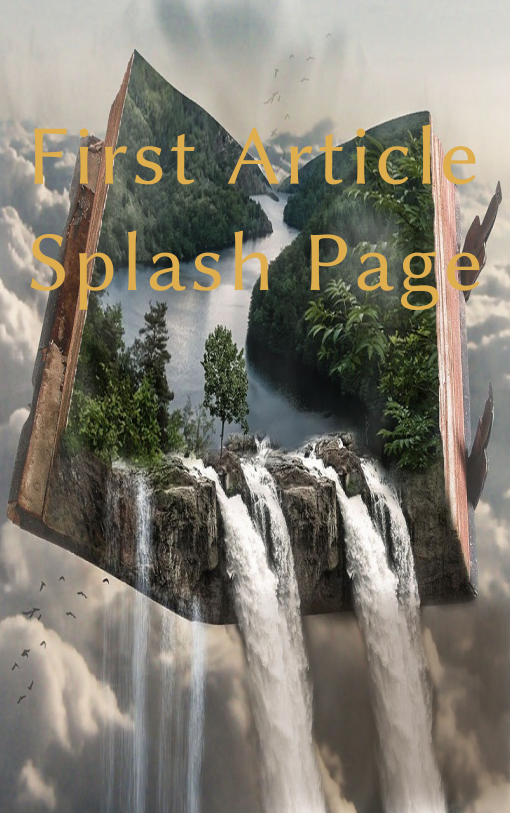
\includegraphics[width=\paperwidth]{./media/images/article_splash}
\end{textblock*}
\clearpage
\chapter{New Horizons\\ \small{Artificial Intelligence For Engaging World Models}}
\begin{figure*}[h]                                                           
 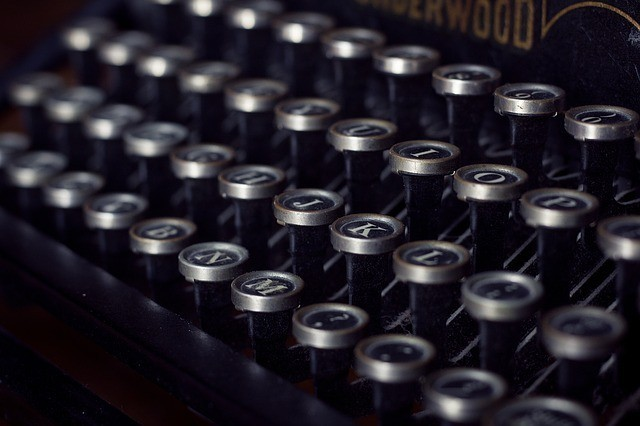
\includegraphics[width=\linewidth]{./media/images/article_lead_image}%
  \scriptsize{\textsc{\\This is} the article main image caption.}
  \label{fig:editorial}%                                                 
\end{figure*}                                                                
\begin{quotation} 
\noindent\color{Sepia}{{\textit{\textbf{“This is the article quote. Now is the
        time for all good men to come to the aid of their country.”}}}}\\[.5mm]
   \hfill\color{Sepia}{\small{\textendash Quotation Author}}
\end{quotation} 
\marginnote{Editor's note: margin notes in red signify links pointing to sites of reference}[2em]
\lettrine[lines=3]{\color{BrickRed}T}{\enspace his is} the first sentence.\reversemarginpar\marginnote{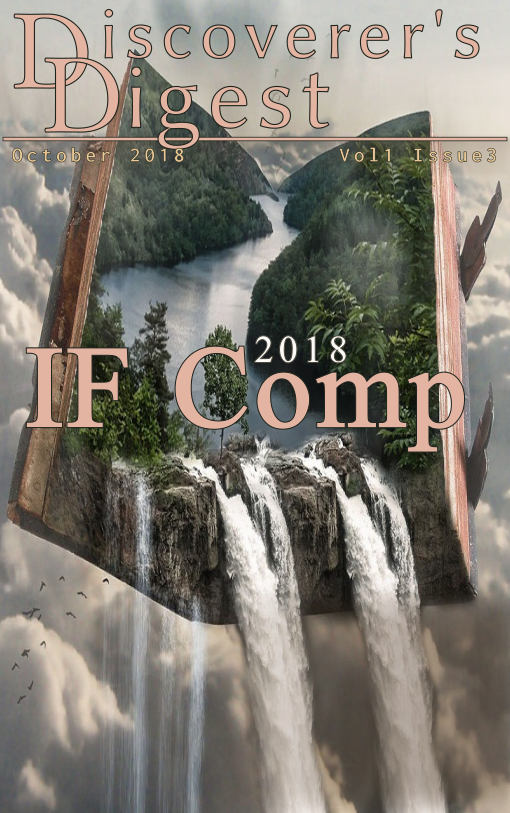
\includegraphics[width=\linewidth]{./media/images/cover}\href{https://www.youtube.com/watch?v=NJarxpYyoFI}{\\This is the marginnote caption(linked)}}
I hope you enjoy this magazine. \emph{Discoverer's Digest } seeks to cover all manner of
topics related to Interactive Fiction, ranging from parser experiences to
choice\textemdash games, along with experiments in the medium (including General Artificial Intelligence) that we've not yet seen.

And please submit your news, story ideas, and comments by sending a personal email to \href{mailto:cooper@discdigest.xyz}{cooper@discdigest.xyz}. \\ \\

\noindent Happy Writing! \\ \\

\noindent \href{mailto:cooper@discdigest.xyz}{\textsc{D. Cooper Stevenson}}


% \chapter*{}
%  \begin{textblock*}{70.9mm}(0mm,0mm)
%    \includegraphics[width=\paperwidth]{./media/images/nltk_cover}
%  \end{textblock*}
%  \chapter{Narrative Intelligence\\ \small{Creating Responsive IF Using NLTK}}
%  \input{./nltk.tex}

% \chapter*{}
%  \begin{textblock*}{70.9mm}(0mm,0mm)
%    \includegraphics[width=\paperwidth]{./media/images/topic_cover}
%  \end{textblock*}
%  \chapter{Topic Modeling\\ \small{Finding Related Topics For Your World Using Gensim}}
% \label{sec:topic}
% \input{./topic.tex}

% \chapter*{}
% \begin{textblock*}{70.9mm}(0mm,0mm)
% \includegraphics[width=\paperwidth]{./media/images/type}
% \end{textblock*}

% \chapter{Epilogue\\ \small{Standing On The Shoulders of Giants}}
% \label{ch:epilogue}
% \input{./epilogue.tex}

% print page notes
\printpagenotes
\end{document}
% Author's Margin Credit
% \marginnote{\includegraphics[width=\linewidth]{/tmp/felice}\href{https://en.wikipedia.org/wiki/Republic_(Plato)}{\\\\By Felicity Banks}}

% Author's Bio
% \begin{wrapfigure}{l}{.25\textwidth}
%   \vspace{-20pt}
%   \begin{center}
%      \includegraphics[width=0.25\textwidth]{/tmp/felice}
%      \caption*{\href{http://cooper.stevenson.name}{\textit{Felicity Banks}}}
%      % } % end parbox
%     \end{center}
%  \end{wrapfigure} 
%\noindent \textit{Banks’ evocation, and then subversion and manipulation, of small details of Australian colonial history is clever and got me checking (historical) names and details on more than one occasion. The story’s action is fast-paced & drives the plot forward with a precision akin to the machinery it embraces.} \\ \\

